\begin{figure}[!htb]
\centering
\begin{subfigure}[t]{0.48\linewidth}
  \centering
  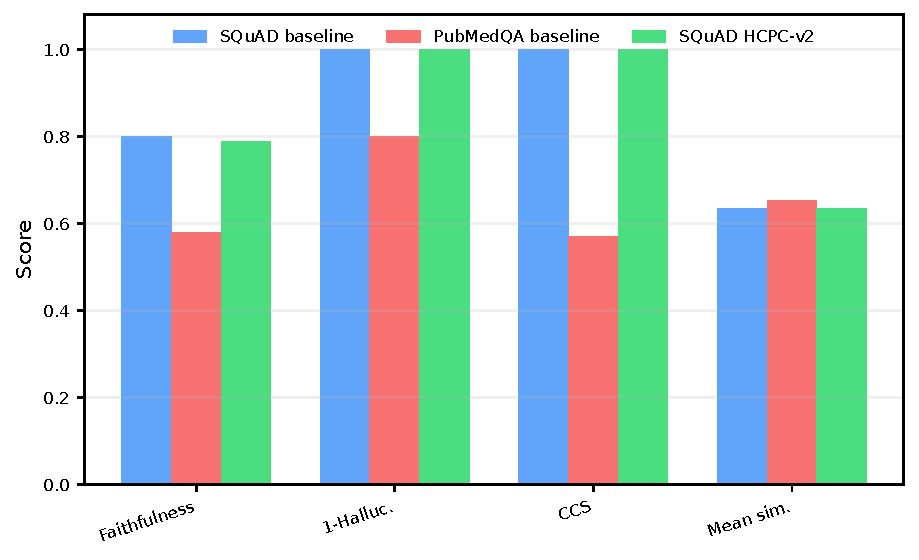
\includegraphics[width=\linewidth]{dataset_comparison.pdf}
  \caption{Dataset-level contrast. PubMedQA achieves comparable retrieval similarity to SQuAD but much worse coherence and hallucination rates.}
  \label{fig:dataset_comparison}
\end{subfigure}
\hfill
\begin{subfigure}[t]{0.48\linewidth}
  \centering
  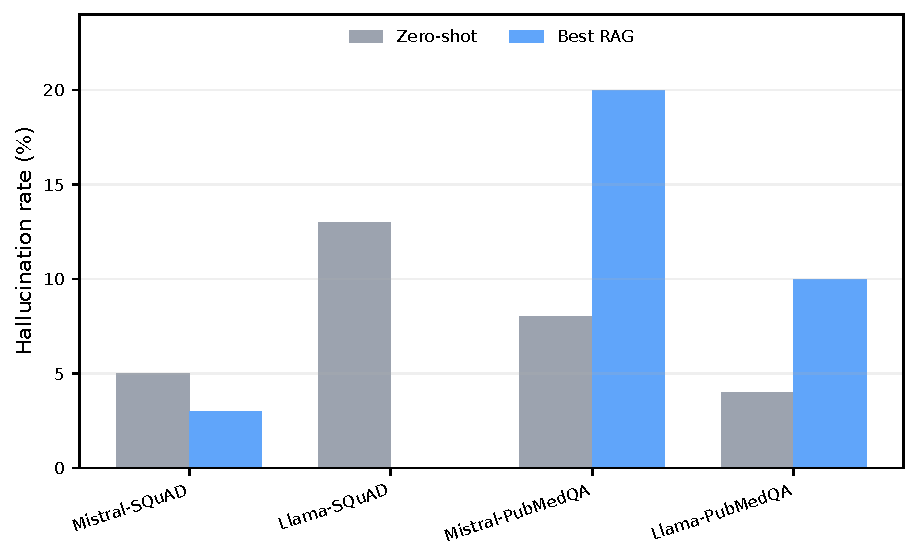
\includegraphics[width=\linewidth]{zeroshot_comparison.pdf}
  \caption{Zero-shot vs.\ best RAG hallucination rates. Retrieval helps on SQuAD but harms on PubMedQA.}
  \label{fig:zeroshot}
\end{subfigure}
\caption{Domain mismatch makes RAG counterproductive. (a)~Local retrieval scores alone do not characterize answer reliability: PubMedQA matches SQuAD on similarity but diverges sharply on coherence and hallucination. (b)~On PubMedQA, the general-domain retriever introduces noisy biomedical evidence that the generator cannot reconcile, making RAG less faithful than zero-shot prompting for both models.}
\label{fig:domain_mismatch_combined}
\end{figure}
